\documentclass[11pt,a4paper]{article}

% =====================================================
% PACKAGES
% =====================================================
\usepackage[utf8]{inputenc}
\usepackage[T1]{fontenc}
\usepackage[french]{babel}
\usepackage{lmodern}
\usepackage{geometry}
\usepackage{xcolor}
\usepackage{graphicx}
\usepackage{booktabs}
\usepackage{tabularx}
\usepackage{array}
\usepackage{float}
\usepackage{hyperref}
\usepackage{listings}
\usepackage{fancyhdr}
\usepackage{titlesec}
\usepackage{enumitem}

\geometry{
    top=2.1cm,
    bottom=2.1cm,
    left=2.3cm,
    right=2.3cm
}

\definecolor{mainblue}{HTML}{163A59}
\definecolor{lightgray}{HTML}{F3F5F7}
\definecolor{codegreen}{HTML}{287C46}

\hypersetup{
    colorlinks=true,
    linkcolor=mainblue,
    urlcolor=mainblue
}

\titleformat{\section}
{\Large\bfseries\color{mainblue}}
{\thesection}{0.7em}{}

\titleformat{\subsection}
{\large\bfseries}
{\thesubsection}{0.7em}{}

\lstdefinestyle{terminal}{
    basicstyle=\ttfamily\footnotesize,
    backgroundcolor=\color{lightgray},
    frame=single,
    rulecolor=\color{gray!35},
    breaklines=true,
    columns=fullflexible,
    keepspaces=true,
    showstringspaces=false,
    keywordstyle=\color{codegreen},
    xleftmargin=5pt,
    xrightmargin=5pt
}

\lstset{style=terminal}

\pagestyle{fancy}
\fancyhf{}
\lhead{\small Infrastructure Windows Server}
\rhead{\small AD DS -- DNS -- SMB -- OT--IT}
\cfoot{\thepage}
\setlength{\headheight}{14pt}

% =====================================================
% DOCUMENT
% =====================================================

\begin{document}

\begin{titlepage}
    \centering
    \vspace*{3cm}

    {\Huge\bfseries
    Infrastructure Windows Server 2022\\[0.3cm]
    Active Directory / OT--IT
    \par}

    \vspace{1cm}

    {\Large
    Mise en place du serveur \texttt{SRV-LAB} et integration du poste TIA
    \par}

    \vspace{1.5cm}

    {\large
    VMware VMnet2 -- AD DS -- DNS -- SMB -- GPO -- Validation poste industriel
    \par}

    \vfill

    \begin{tabular}{rl}
        Serveur : & \texttt{SRV-LAB} \\
        Domaine : & \texttt{ad.lab} \\
        Reseau OT : & \texttt{192.168.161.0/24} \\
        Date des captures : & Octobre 2026 \\
    \end{tabular}

    \vspace{2cm}

    {\large Documentation technique prete pour Overleaf et GitHub}

\end{titlepage}

\tableofcontents
\newpage

% =====================================================
\section{Objectif du document}
% =====================================================

Ce document decrit l'infrastructure Windows Server mise en place pour
le laboratoire OT--IT : creation de la VM serveur, reseau VMware
\texttt{VMnet2}, configuration IP, Active Directory Domain Services,
DNS, organisation des OU, utilisateurs et groupes, partage SMB, droits
NTFS, integration de la VM Siemens TIA Portal et GPO d'administration
locale.

Il complete le document separe consacre a la VM Siemens TIA Portal.
Les projets Ignition et AVEVA sont prevus pour plus tard et ne sont pas
presentes comme installes.

% =====================================================
\section{Architecture generale}
% =====================================================

\subsection{Plan reseau}

\begin{lstlisting}
PC hote Windows / VMware
  |
  +-- VMnet8 NAT
  |     +-- Acces Internet des VM
  |
  +-- VMnet2 Host-only / OT-Lab
        Sous-reseau : 192.168.161.0/24
        DHCP       : desactive
        Hote       : 192.168.161.1
        |
        +-- SRV-LAB / ad.lab / DNS
        |     IP : 192.168.161.10
        |
        +-- VM Siemens TIA Portal
              IP : 192.168.161.20
              DNS : 192.168.161.10
\end{lstlisting}

\subsection{Roles}

\begin{table}[H]
\centering
\begin{tabularx}{\textwidth}{lX}
\toprule
\textbf{Element} & \textbf{Role} \\
\midrule
VMware VMnet2 & Reseau OT prive entre le serveur et le poste Siemens. \\
\texttt{SRV-LAB} & Controleur de domaine, DNS et serveur de fichiers. \\
\texttt{ad.lab} & Domaine Active Directory du laboratoire. \\
VM Siemens & Poste d'ingenierie TIA Portal joint au domaine. \\
\texttt{Projets\_Automatisme} & Partage SMB de travail pour les projets. \\
\texttt{GPO\_Admins\_Locaux\_Postes} & GPO ajoutant un groupe AD dans les administrateurs locaux des postes. \\
\bottomrule
\end{tabularx}
\caption{Role des composants de l'infrastructure}
\end{table}

% =====================================================
\section{Creation de la VM Windows Server}
% =====================================================

\subsection{Assistant VMware}

La VM serveur a ete creee avec l'assistant VMware Workstation. La capture
montre la compatibilite materielle \og Workstation 25H2 or later \fg{}.

\begin{figure}[H]
    \centering
    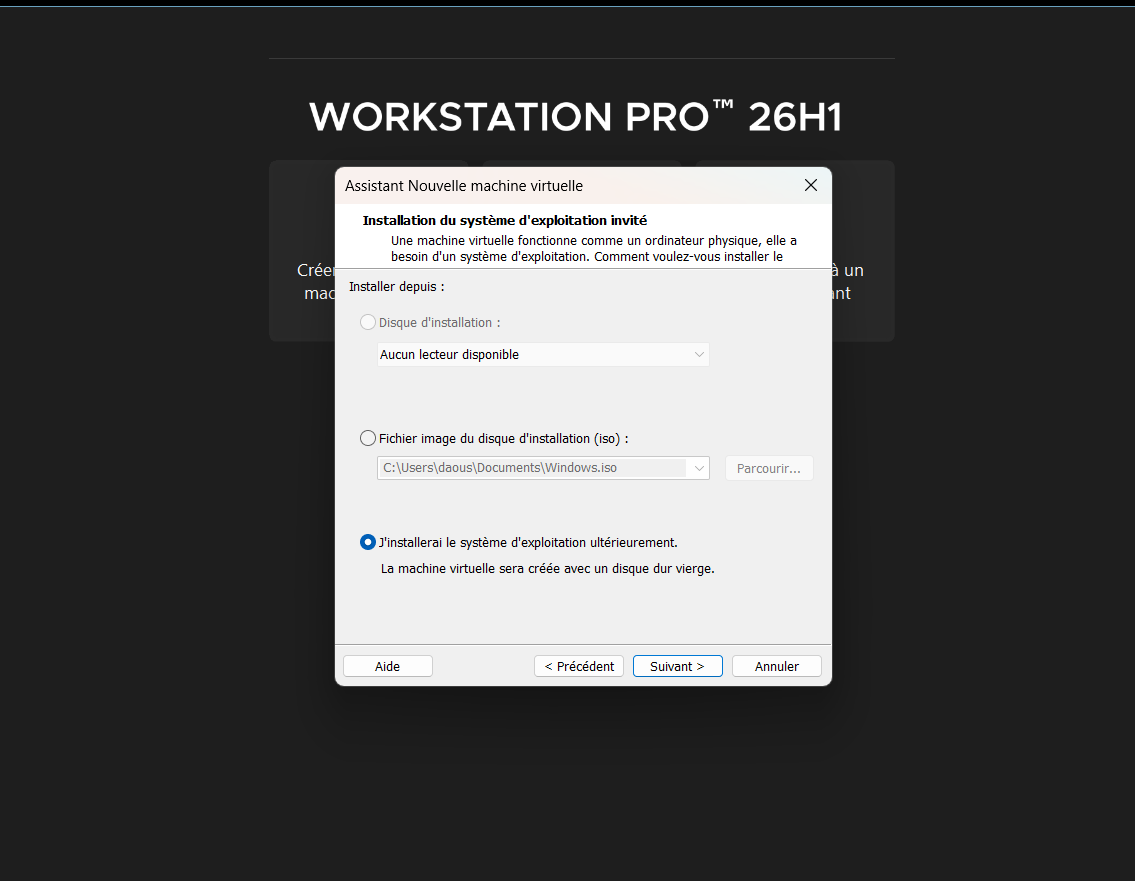
\includegraphics[width=0.62\textwidth]{images/srv-01-vmware-compatibilite-materielle.png}
    \caption{Creation de la VM serveur dans VMware Workstation.}
\end{figure}

Le disque virtuel observe porte le nom
\texttt{Windows\_Server\_2022\_SCADA.vmdk}. Le nom initial visible dans
les captures etait oriente SCADA, puis le serveur a ete renomme
\texttt{SRV-LAB}.

\begin{figure}[H]
    \centering
    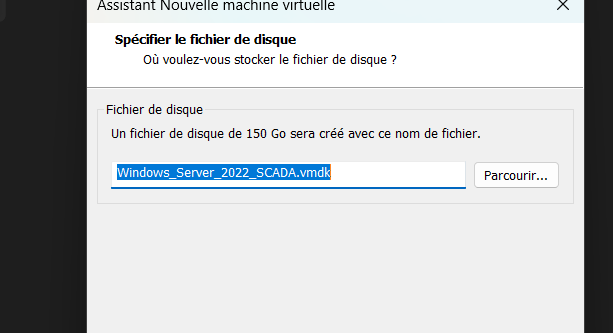
\includegraphics[width=0.70\textwidth]{images/srv-02-vmware-disque-windows-server.png}
    \caption{Disque virtuel associe a la VM Windows Server 2022.}
\end{figure}

\subsection{Installation Windows Server}

L'installation Windows Server a ete lancee dans la VM. Les captures
montrent l'assistant Microsoft puis l'arrivee sur Server Manager.

\begin{figure}[H]
    \centering
    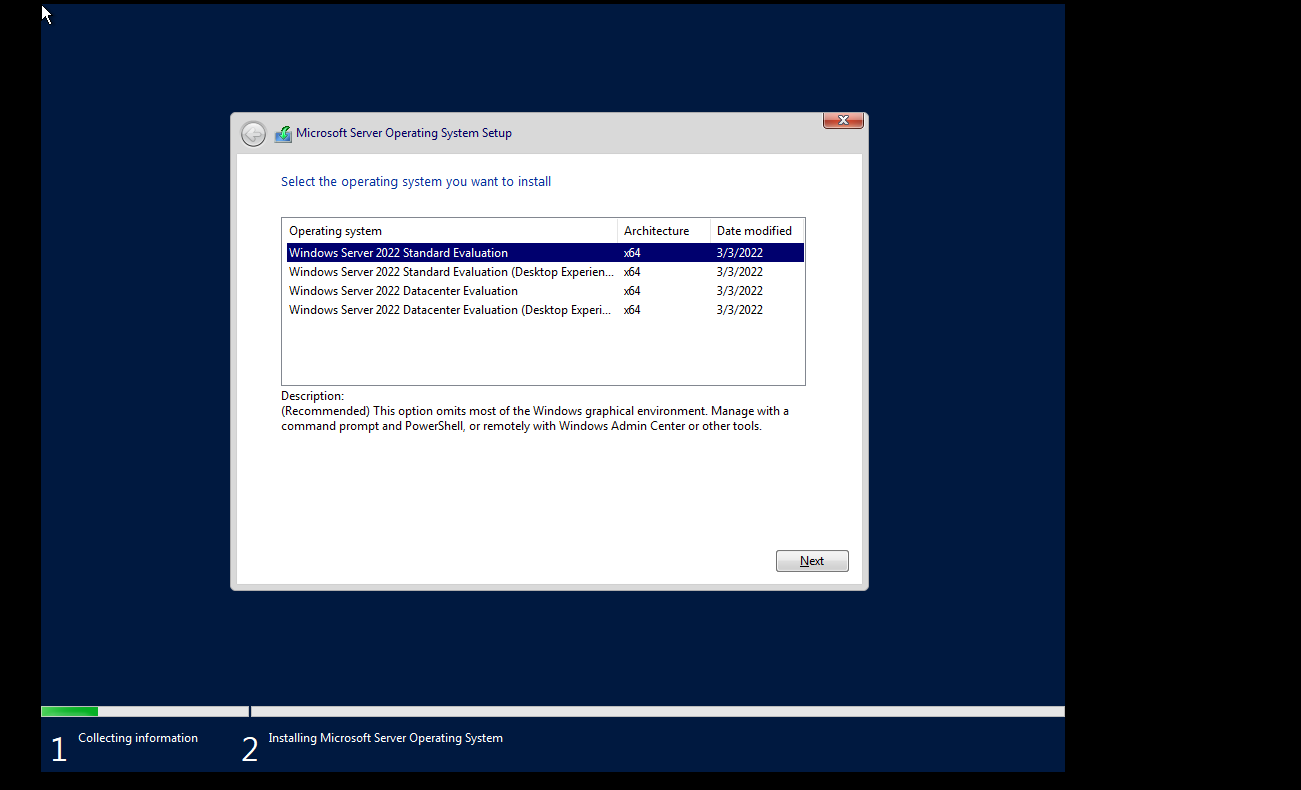
\includegraphics[width=0.72\textwidth]{images/srv-03-installation-windows-server.png}
    \caption{Assistant d'installation Windows Server dans la VM.}
\end{figure}

\begin{figure}[H]
    \centering
    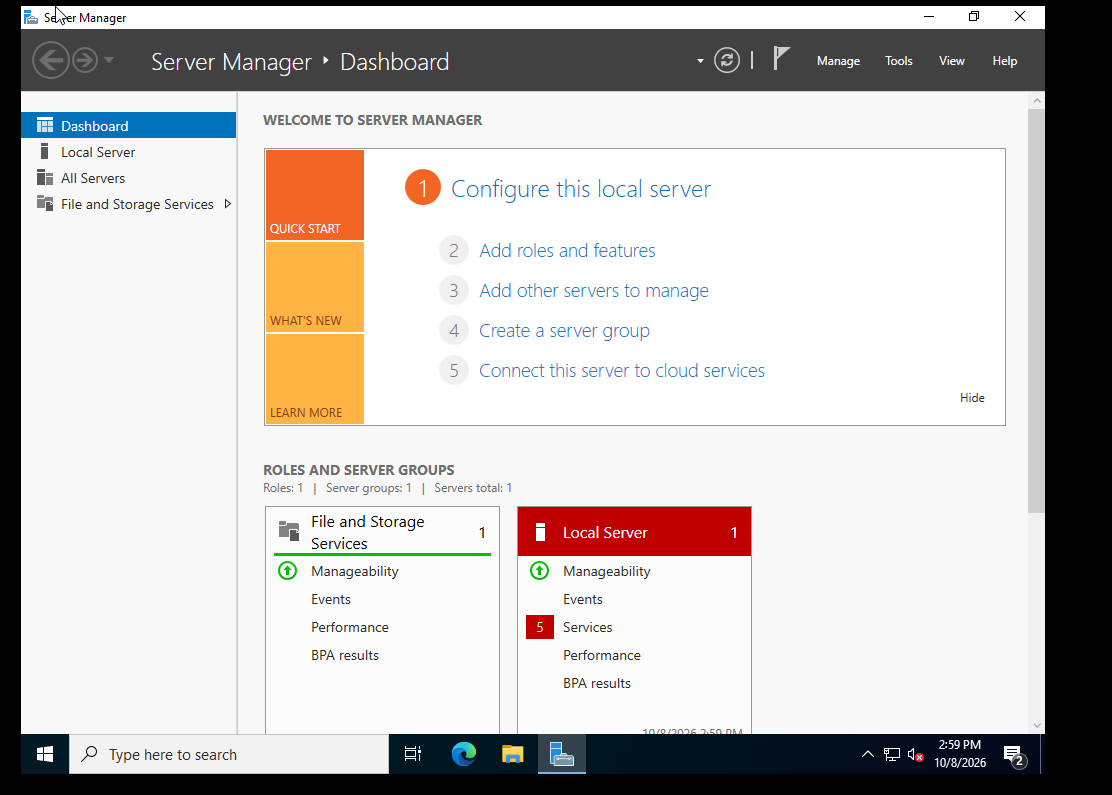
\includegraphics[width=0.85\textwidth]{images/srv-04-server-manager-dashboard.png}
    \caption{Server Manager apres installation de Windows Server.}
\end{figure}

% =====================================================
\section{Reseau VMware VMnet2}
% =====================================================

\subsection{Configuration du reseau OT}

Le reseau \texttt{VMnet2} est configure en mode Host-only. La connexion
a l'adaptateur virtuel de l'hote est activee, le service DHCP local est
desactive et le sous-reseau est \texttt{192.168.161.0/24}.

\begin{figure}[H]
    \centering
    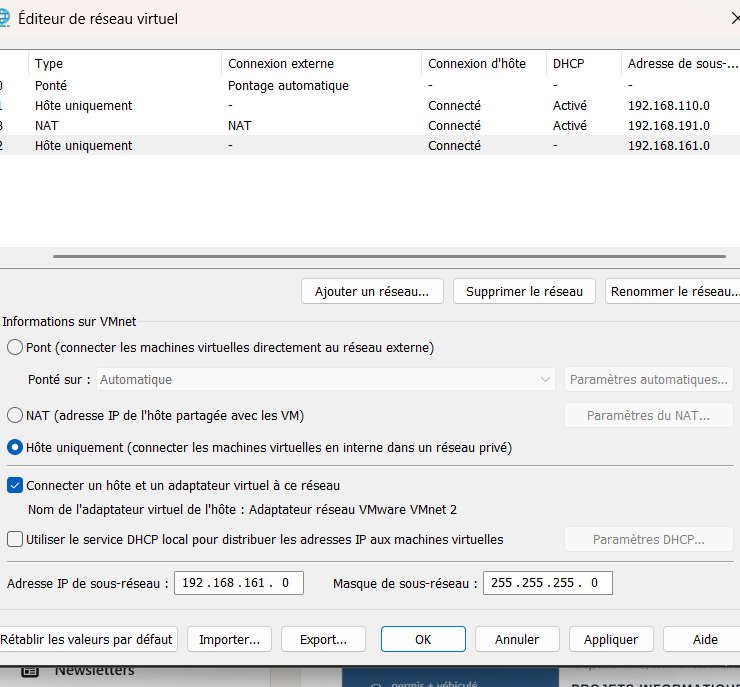
\includegraphics[width=\textwidth]{images/srv-05-vmnet2-host-only-dhcp-off.png}
    \caption{VMnet2 en Host-only, DHCP desactive, sous-reseau 192.168.161.0/24.}
\end{figure}

\subsection{Adresse cote hote}

L'adaptateur \texttt{VMware Network Adapter VMnet2} du PC hote utilise
l'adresse \texttt{192.168.161.1/24}. Aucune passerelle n'est definie sur
ce reseau prive.

\begin{figure}[H]
    \centering
    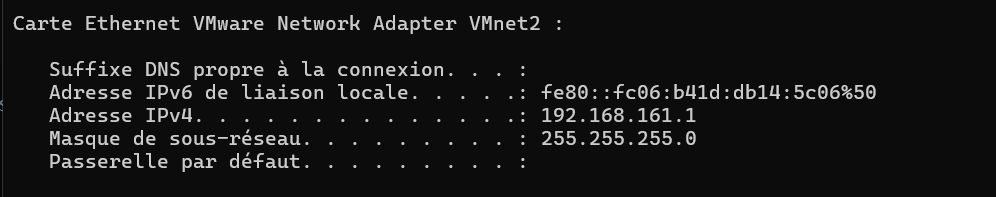
\includegraphics[width=0.84\textwidth]{images/srv-06-hote-vmnet2-ip-192-168-161-1.png}
    \caption{Adresse IPv4 du PC hote sur VMnet2.}
\end{figure}

% =====================================================
\section{Configuration de SRV-LAB}
% =====================================================

\subsection{Adresse IP statique}

Le serveur utilise l'adresse \texttt{192.168.161.10/24} sur le reseau
OT. La capture montre l'IP statique sans passerelle.

\begin{figure}[H]
    \centering
    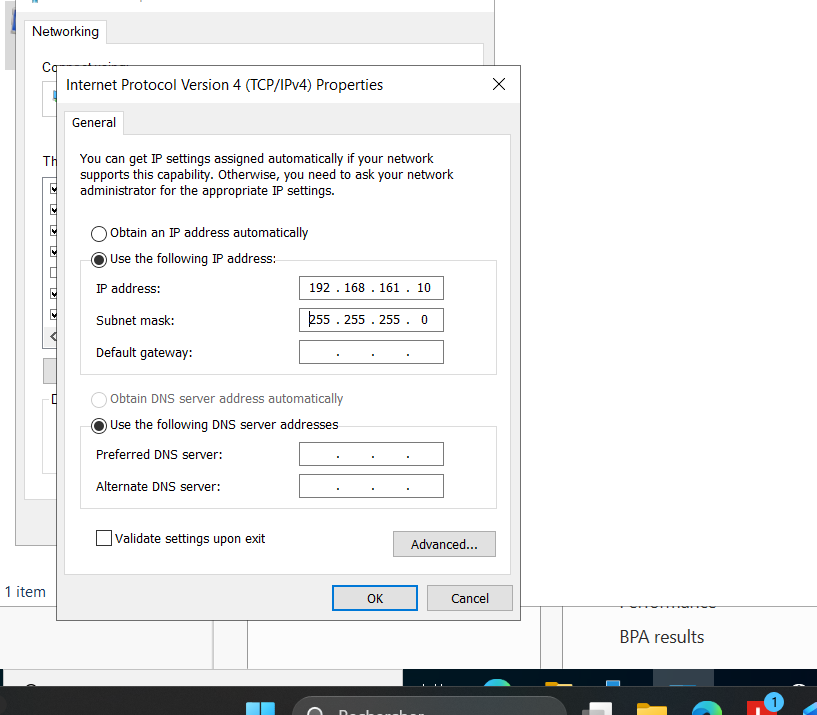
\includegraphics[width=0.70\textwidth]{images/srv-07-srv-lab-ip-192-168-161-10.png}
    \caption{Configuration IPv4 statique du serveur SRV-LAB.}
\end{figure}

\subsection{Renommage du serveur}

La commande suivante a ete utilisee pour renommer le serveur :

\begin{lstlisting}
Rename-Computer -NewName "SRV-LAB"
\end{lstlisting}

Le redemarrage etait necessaire pour appliquer le changement.

\begin{figure}[H]
    \centering
    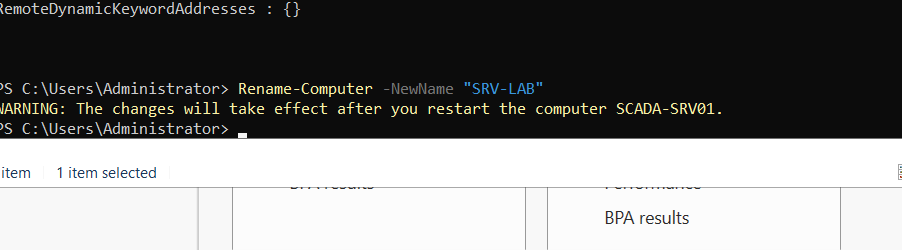
\includegraphics[width=0.82\textwidth]{images/srv-08-renommage-srv-lab.png}
    \caption{Renommage du serveur en SRV-LAB.}
\end{figure}

% =====================================================
\section{Active Directory et DNS}
% =====================================================

\subsection{Installation AD DS}

Le role Active Directory Domain Services a ete ajoute depuis Server
Manager. Le serveur cible visible dans l'assistant est
\texttt{SRV-LAB}.

\begin{figure}[H]
    \centering
    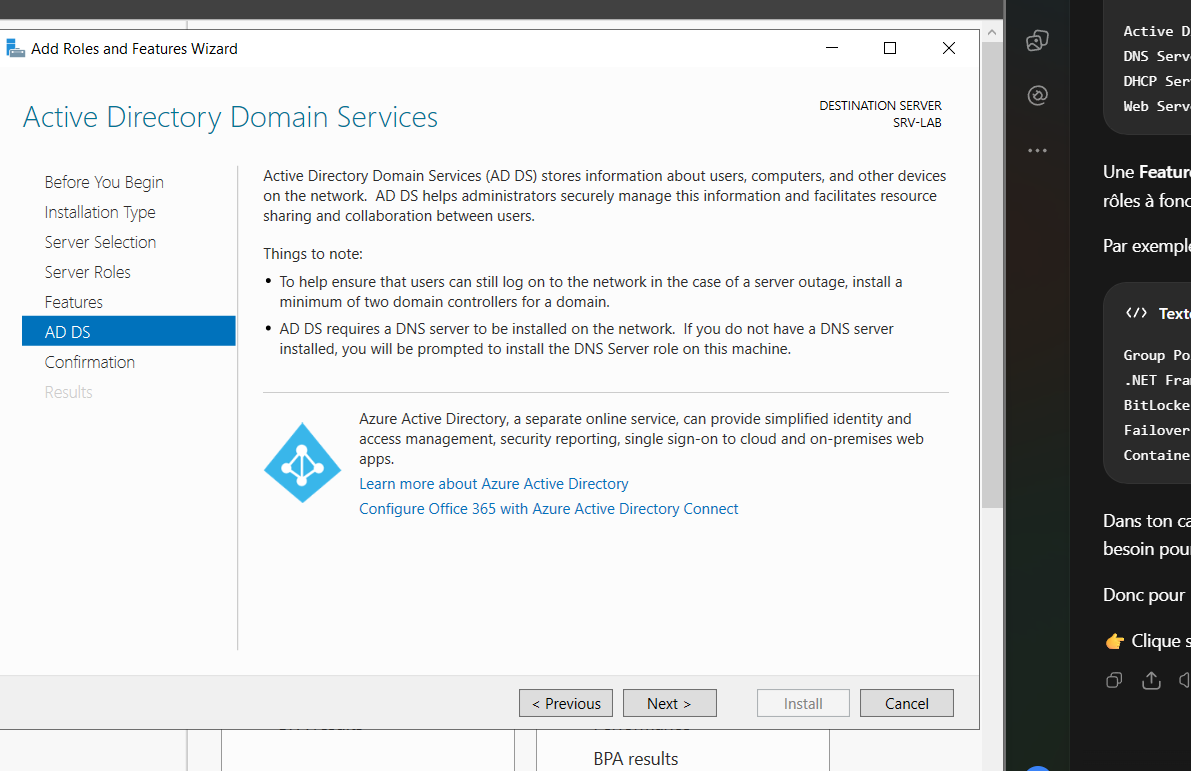
\includegraphics[width=0.82\textwidth]{images/srv-09-role-ad-ds.png}
    \caption{Ajout du role Active Directory Domain Services.}
\end{figure}

\subsection{Promotion et DNS}

Le domaine cree est \texttt{ad.lab}. Pendant la promotion, un avertissement
DNS concernant la delegation est apparu. Dans un laboratoire local sans
zone parente publique, cet avertissement est attendu et n'a pas bloque
la creation du domaine.

\begin{figure}[H]
    \centering
    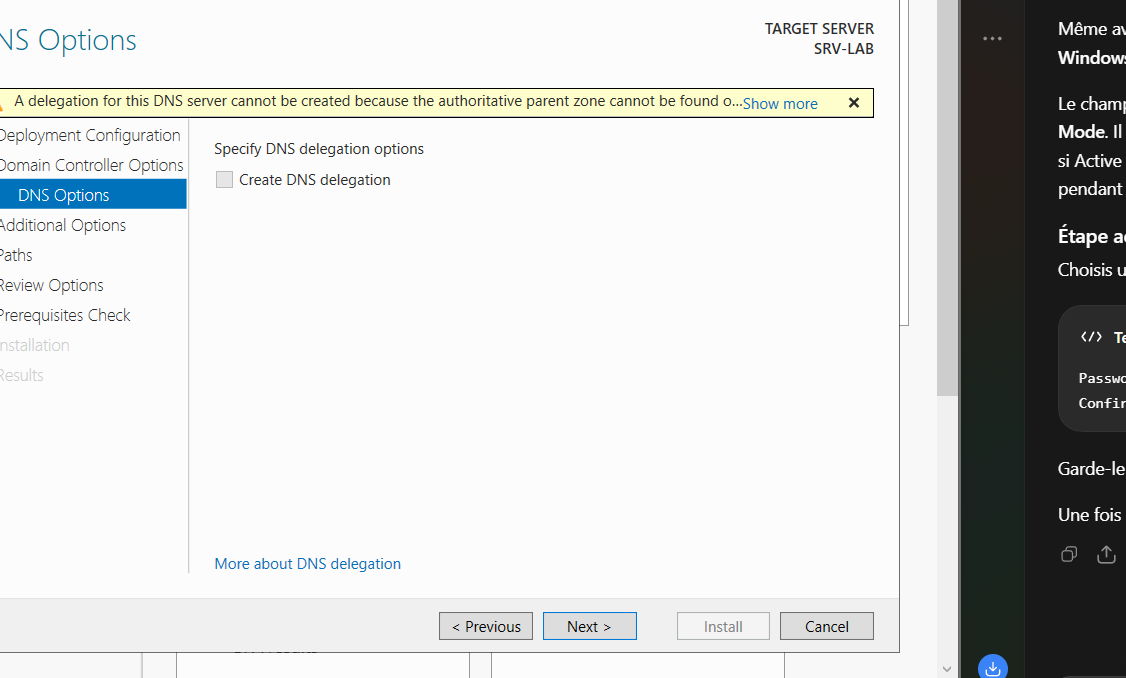
\includegraphics[width=0.82\textwidth]{images/srv-10-dns-warning-delegation.png}
    \caption{Avertissement de delegation DNS pendant la promotion du serveur.}
\end{figure}

La resolution DNS du domaine a ete validee par :

\begin{lstlisting}
nslookup ad.lab
\end{lstlisting}

Le resultat observe renvoie \texttt{ad.lab} vers \texttt{192.168.161.10}.

\begin{figure}[H]
    \centering
    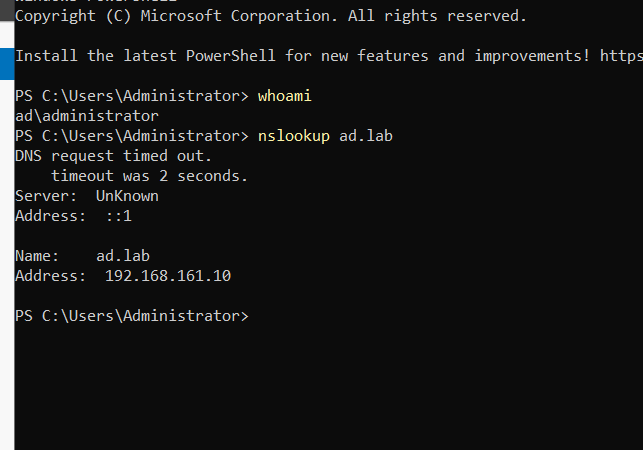
\includegraphics[width=0.74\textwidth]{images/srv-11-validation-dns-ad-lab.png}
    \caption{Validation DNS du domaine ad.lab vers 192.168.161.10.}
\end{figure}

\subsection{Controle DNS local}

Une verification utile cote serveur est :

\begin{lstlisting}
Get-DnsClientServerAddress
\end{lstlisting}

Dans les captures, l'interface IPv4 utilise \texttt{127.0.0.1}, ce qui
correspond au role DNS local du controleur de domaine.

% =====================================================
\section{OU, utilisateurs et groupes}
% =====================================================

\subsection{Structure Active Directory}

La console Active Directory Users and Computers confirme le domaine
\texttt{ad.lab}. Des OU de laboratoire ont ensuite ete creees pour
separer les utilisateurs, groupes, administrateurs et postes industriels.

\begin{figure}[H]
    \centering
    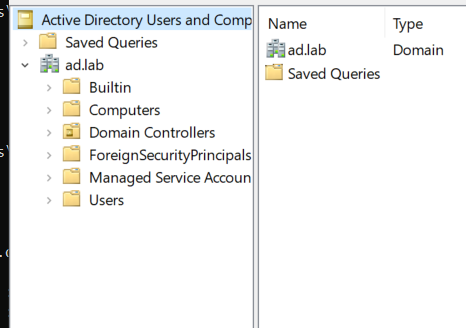
\includegraphics[width=0.60\textwidth]{images/srv-12-aduc-domaine-ad-lab.png}
    \caption{Domaine ad.lab visible dans Active Directory Users and Computers.}
\end{figure}

Une capture montre la creation d'un utilisateur dans l'OU
\texttt{LAB\_Utilisateurs}. Les champs personnels ne sont pas repris dans
ce document.

\begin{figure}[H]
    \centering
    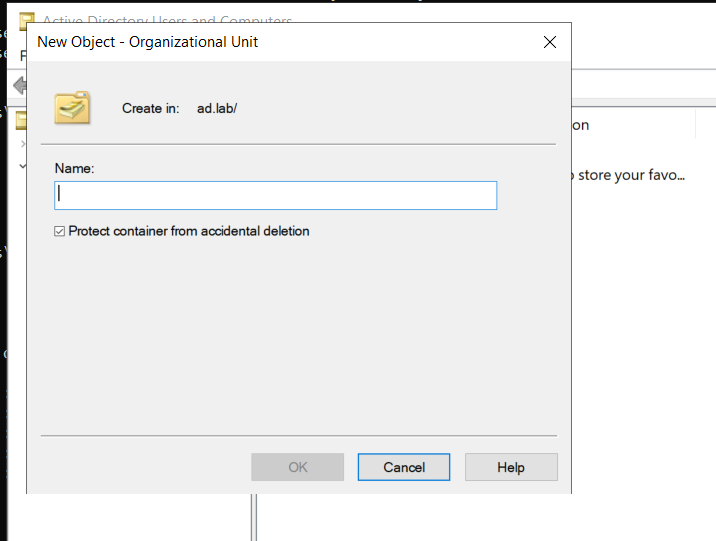
\includegraphics[width=0.70\textwidth]{images/srv-13-creation-ou-utilisateurs.png}
    \caption{Creation d'objet utilisateur dans l'OU LAB Utilisateurs.}
\end{figure}

\subsection{Noms fonctionnels retenus}

Les noms suivants sont utilises dans la documentation :

\begin{itemize}[leftmargin=*]
    \item \texttt{LAB\_Utilisateurs} ;
    \item \texttt{LAB\_Groupes} ;
    \item \texttt{LAB\_Administrateurs} ;
    \item \texttt{LAB\_Postes\_Industriels} ;
    \item \texttt{GG\_Automaticiens} ;
    \item \texttt{GG\_Admins\_Postes}.
\end{itemize}

% =====================================================
\section{Partage SMB et droits NTFS}
% =====================================================

\subsection{Dossier partage}

Le dossier de travail est :

\begin{lstlisting}
C:\LAB\Projets_Automatisme
\end{lstlisting}

Il est partage sous le nom :

\begin{lstlisting}
\\192.168.161.10\Projets_Automatisme
\end{lstlisting}

\subsection{Droits NTFS}

Le groupe \texttt{AD\textbackslash GG\_Automaticiens} a ete ajoute dans
les permissions NTFS du dossier, avec des droits de modification.

\begin{figure}[H]
    \centering
    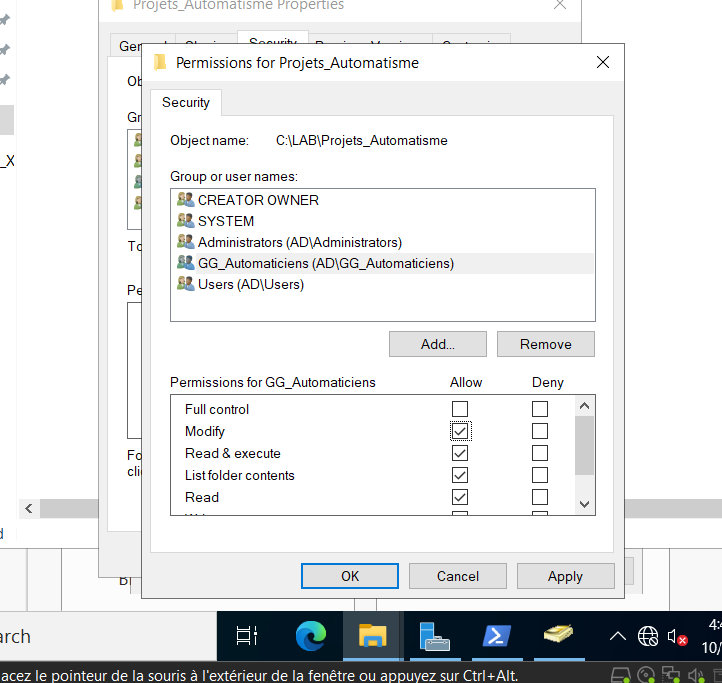
\includegraphics[width=0.58\textwidth]{images/srv-14-ntfs-groupe-automaticiens.png}
    \caption{Ajout du groupe GG Automaticiens dans les permissions NTFS.}
\end{figure}

\subsection{Droits de partage}

Le partage SMB donne le droit \og Change \fg{} au groupe
\texttt{GG\_Automaticiens}. Les administrateurs du domaine gardent un
controle complet.

\begin{figure}[H]
    \centering
    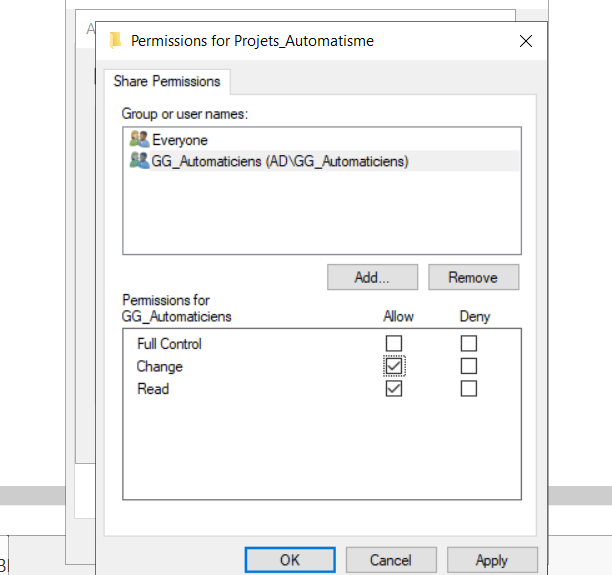
\includegraphics[width=0.58\textwidth]{images/srv-15-partage-smb-droits-change.png}
    \caption{Droits de partage SMB pour GG Automaticiens.}
\end{figure}

La commande de validation cote serveur est :

\begin{lstlisting}
Get-SmbShareAccess -Name "Projets_Automatisme"
\end{lstlisting}

Le resultat observe indique :

\begin{lstlisting}
AD\Domain Admins      Allow  Full
AD\GG_Automaticiens   Allow  Change
\end{lstlisting}

\begin{figure}[H]
    \centering
    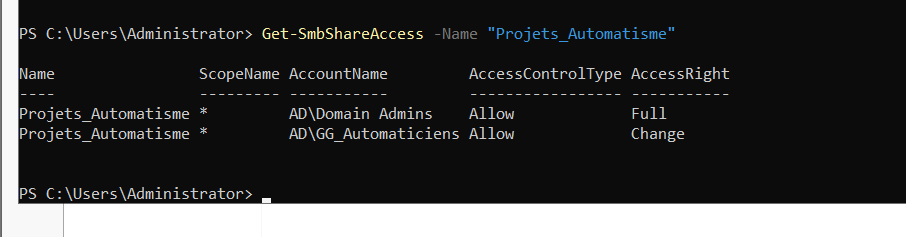
\includegraphics[width=0.82\textwidth]{images/srv-16-get-smb-share-access.png}
    \caption{Validation PowerShell des droits de partage SMB.}
\end{figure}

\subsection{Diagnostic reseau SMB}

Le port SMB 445 du serveur a ete teste depuis le PC hote :

\begin{lstlisting}
Test-NetConnection 192.168.161.10 -Port 445
\end{lstlisting}

Le resultat \texttt{TcpTestSucceeded : True} valide l'accessibilite du
service SMB sur le reseau VMnet2.

\begin{figure}[H]
    \centering
    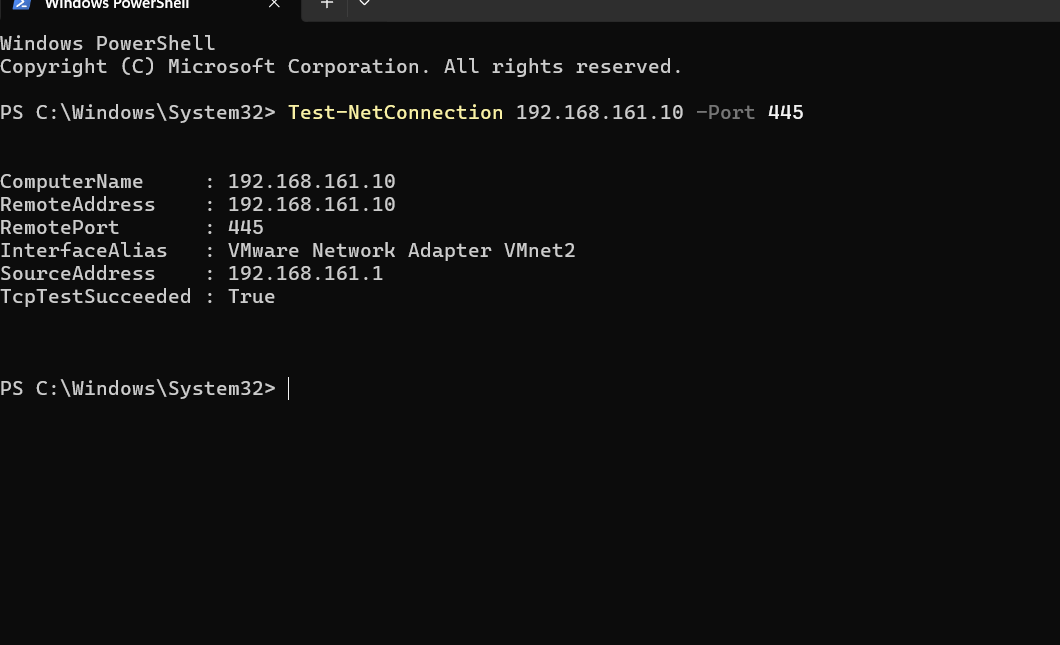
\includegraphics[width=0.82\textwidth]{images/srv-17-test-port-smb-445.png}
    \caption{Test du port SMB 445 vers SRV-LAB.}
\end{figure}

% =====================================================
\section{Integration de la VM Siemens}
% =====================================================

\subsection{Adresse IP de la VM TIA}

La VM Siemens dispose de deux cartes reseau : une carte NAT pour Internet
et une carte VMnet2 pour le reseau OT. Sur VMnet2, l'adresse configuree
est \texttt{192.168.161.20/24} avec le DNS \texttt{192.168.161.10}.

\begin{figure}[H]
    \centering
    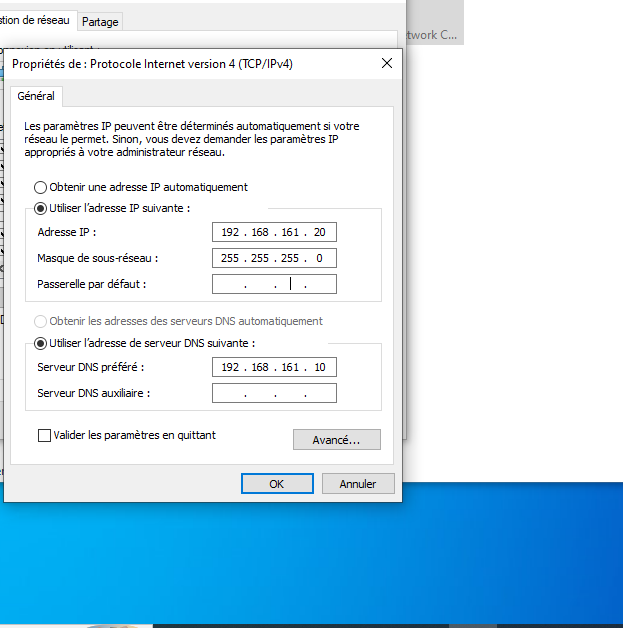
\includegraphics[width=0.54\textwidth]{images/srv-20-tia-vm-ip-192-168-161-20.png}
    \caption{Configuration IPv4 de la carte VMnet2 dans la VM Siemens.}
\end{figure}

\subsection{Acces au partage SMB}

Avant correction des droits, Windows refusait l'acces au partage
\texttt{Projets\_Automatisme}. Cette erreur etait utile : le reseau
fonctionnait, mais les autorisations n'etaient pas encore suffisantes.

\begin{figure}[H]
    \centering
    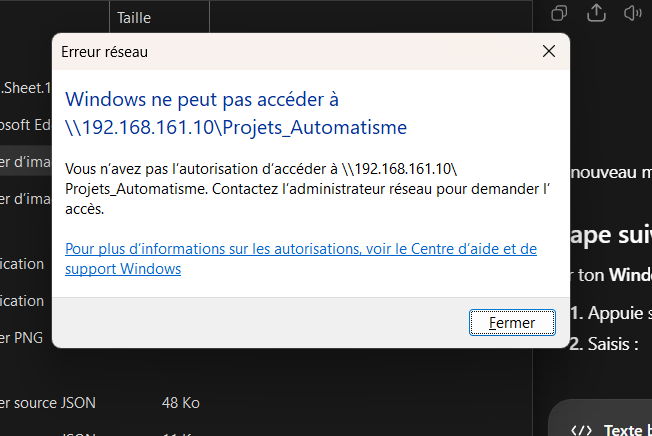
\includegraphics[width=0.62\textwidth]{images/srv-18-erreur-acces-smb-avant-droits.png}
    \caption{Erreur d'autorisation SMB avant correction des droits.}
\end{figure}

Apres correction, la commande suivante renvoie un etat \texttt{OK} :

\begin{lstlisting}
net use
\end{lstlisting}

\begin{figure}[H]
    \centering
    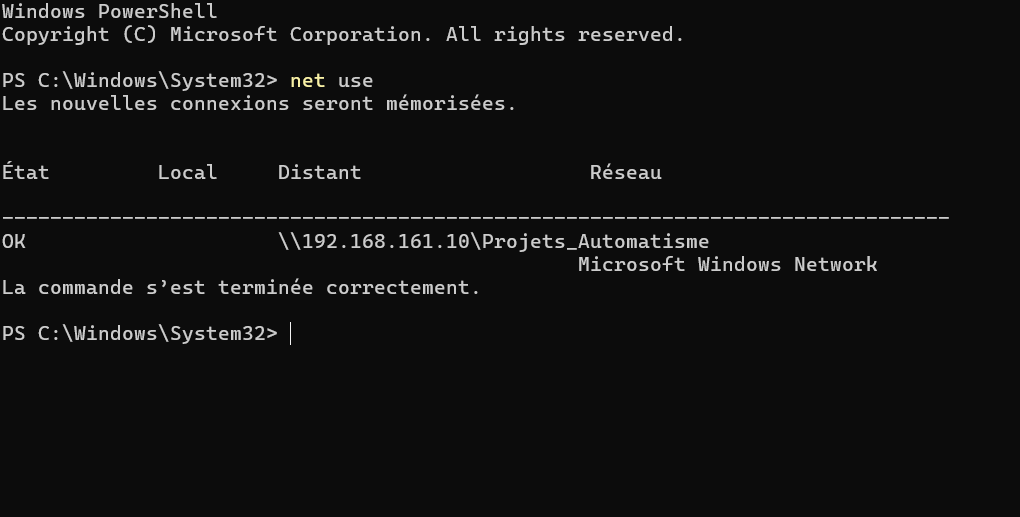
\includegraphics[width=0.76\textwidth]{images/srv-19-net-use-smb-ok.png}
    \caption{Connexion SMB validee vers le partage Projets Automatisme.}
\end{figure}

\subsection{Jonction au domaine}

La VM Siemens a ete jointe au domaine \texttt{ad.lab}. Le nom du poste
observe dans les validations est \texttt{DESKTOP-H6FRU6M}. Pour une
publication GitHub finale, il est possible de remplacer ce nom par un
nom plus generique dans le texte, par exemple \texttt{TIA-POSTE01}.

% =====================================================
\section{GPO d'administration locale}
% =====================================================

\subsection{Objectif}

La GPO \texttt{GPO\_Admins\_Locaux\_Postes} a pour but d'ajouter le
groupe \texttt{AD\textbackslash GG\_Admins\_Postes} au groupe
Administrateurs local des postes industriels.

Cette configuration evite d'ajouter manuellement les administrateurs sur
chaque poste.

\subsection{Ciblage de l'OU}

La console Group Policy Management montre l'OU
\texttt{LAB\_Postes\_Industriels}, destinee a contenir les postes du
laboratoire.

\begin{figure}[H]
    \centering
    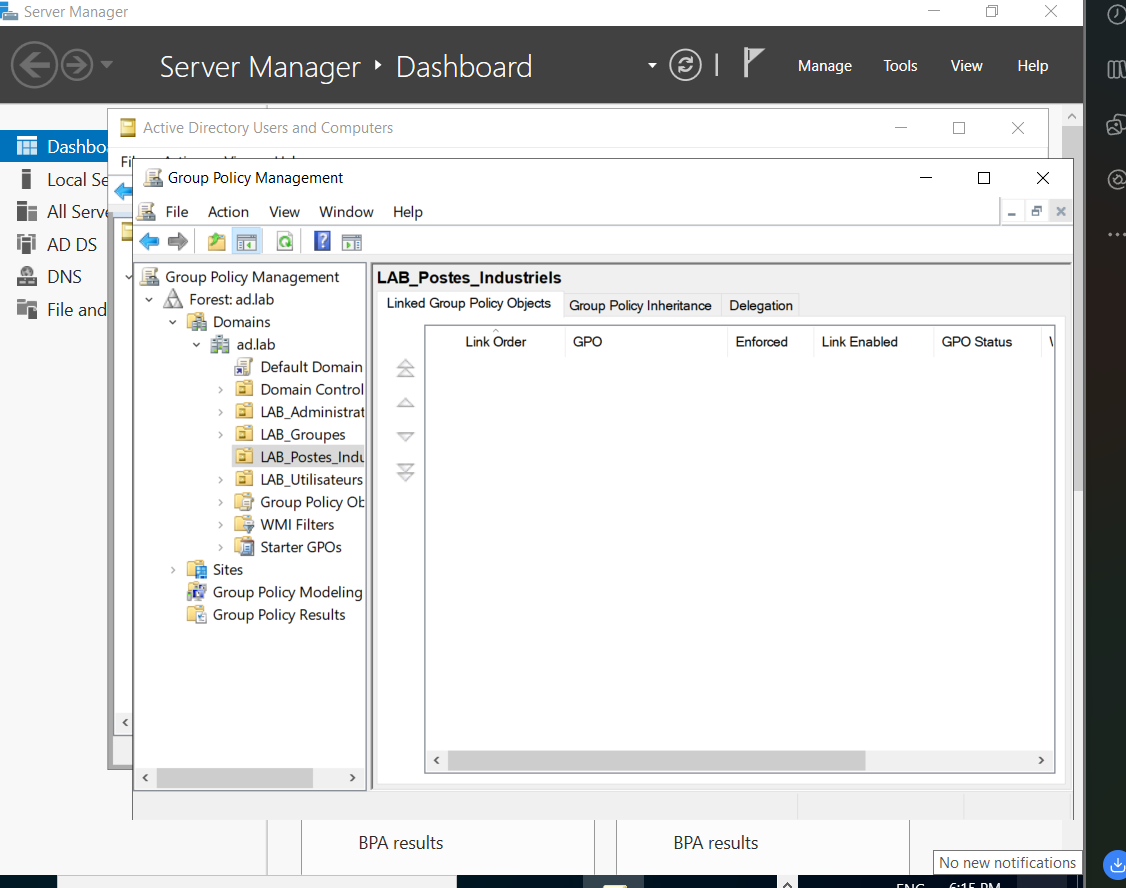
\includegraphics[width=0.84\textwidth]{images/srv-21-gpo-ou-postes-industriels.png}
    \caption{OU LAB Postes Industriels dans Group Policy Management.}
\end{figure}

\subsection{Configuration du groupe local}

La GPO configure le groupe local \og Administrators (built-in) \fg{} et
ajoute \texttt{AD\textbackslash GG\_Admins\_Postes} comme membre.

\begin{figure}[H]
    \centering
    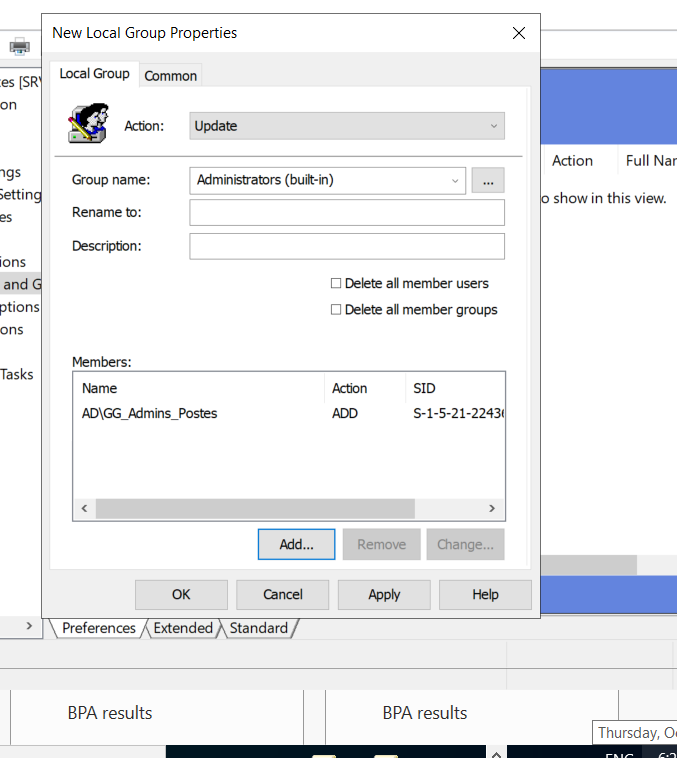
\includegraphics[width=0.62\textwidth]{images/srv-22-gpo-admins-locaux-postes.png}
    \caption{Ajout de GG Admins Postes dans les administrateurs locaux via GPO.}
\end{figure}

\subsection{Application cote poste}

Sur la VM Siemens, la commande suivante a ete lancee :

\begin{lstlisting}
gpupdate /force
\end{lstlisting}

\begin{figure}[H]
    \centering
    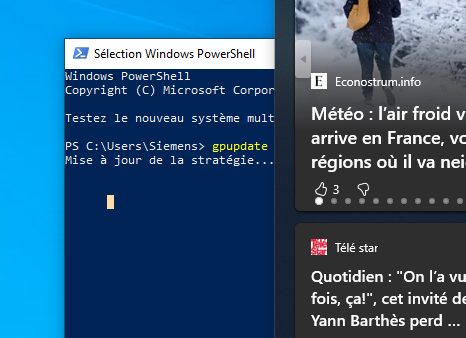
\includegraphics[width=0.58\textwidth]{images/srv-23-gpupdate-poste-tia.png}
    \caption{Mise a jour de strategie de groupe sur le poste TIA.}
\end{figure}

La validation finale fournie dans la conversation est :

\begin{lstlisting}
Get-LocalGroupMember -Group (Get-LocalGroup -SID "S-1-5-32-544").Name

ObjectClass Name                           PrincipalSource
----------- ----                           ---------------
Groupe      AD\Domain Admins               ActiveDirectory
Groupe      AD\GG_Admins_Postes            ActiveDirectory
Utilisateur DESKTOP-H6FRU6M\Administrateur Local
Utilisateur DESKTOP-H6FRU6M\Siemens        Local
\end{lstlisting}

Ce resultat confirme que \texttt{GG\_Admins\_Postes} est bien membre
du groupe Administrateurs local du poste TIA.

% =====================================================
\section{Incidents et corrections}
% =====================================================

\subsection{Avertissement de delegation DNS}

Pendant la promotion AD DS, l'assistant a signale que la delegation DNS
ne pouvait pas etre creee. Dans ce laboratoire, le domaine
\texttt{ad.lab} est local et il n'existe pas de zone parente a deleguer.
L'avertissement a donc ete documente puis l'installation a continue.

\subsection{Acces SMB refuse}

Le premier acces au partage a renvoye une erreur d'autorisation. La
correction a consiste a ajuster les droits NTFS et les droits de partage
pour le groupe \texttt{GG\_Automaticiens}.

\subsection{Resolution DNS}

La resolution de \texttt{ad.lab} vers \texttt{192.168.161.10} a ete
controlee par \texttt{nslookup}. La presence de \texttt{Server: Unknown}
dans la sortie n'empeche pas la resolution ; elle indique seulement que
le nom inverse du serveur DNS n'etait pas renseigne dans cette capture.

% =====================================================
\section{Commandes utiles}
% =====================================================

\begin{lstlisting}
# Renommer le serveur
Rename-Computer -NewName "SRV-LAB"

# Verifier le DNS local
nslookup ad.lab
Get-DnsClientServerAddress

# Verifier le port SMB
Test-NetConnection 192.168.161.10 -Port 445

# Verifier les droits du partage
Get-SmbShareAccess -Name "Projets_Automatisme"

# Verifier les administrateurs locaux sur le poste TIA
Get-LocalGroupMember -Group (Get-LocalGroup -SID "S-1-5-32-544").Name

# Appliquer les GPO sur le poste client
gpupdate /force
\end{lstlisting}

% =====================================================
\section{Bilan des validations}
% =====================================================

\begin{table}[H]
\centering
\begin{tabularx}{\textwidth}{Xc}
\toprule
\textbf{Validation} & \textbf{Resultat} \\
\midrule
VM Windows Server creee dans VMware & OK \\
VMnet2 Host-only en \texttt{192.168.161.0/24} & OK \\
DHCP VMware desactive sur VMnet2 & OK \\
PC hote en \texttt{192.168.161.1} & OK \\
SRV-LAB en \texttt{192.168.161.10} & OK \\
Domaine \texttt{ad.lab} cree & OK \\
DNS \texttt{ad.lab} vers \texttt{192.168.161.10} & OK \\
OU de laboratoire creees & OK \\
Partage SMB \texttt{Projets\_Automatisme} cree & OK \\
Droits SMB et NTFS pour groupes AD & OK \\
VM TIA en \texttt{192.168.161.20} avec DNS serveur & OK \\
Connexion SMB apres correction des droits & OK \\
GPO d'administrateurs locaux appliquee & OK \\
\bottomrule
\end{tabularx}
\caption{Synthese des validations observees}
\end{table}

% =====================================================
\section{Conclusion}
% =====================================================

L'infrastructure Windows Server 2022 du laboratoire est operationnelle
pour les besoins OT--IT actuels. Le serveur \texttt{SRV-LAB} fournit le
domaine \texttt{ad.lab}, le DNS, les OU de laboratoire, les groupes AD,
un partage SMB pour les projets d'automatisme et une GPO permettant de
gerer les administrateurs locaux des postes.

La VM Siemens TIA Portal est integree au reseau OT via
\texttt{VMnet2}, avec une adresse statique \texttt{192.168.161.20} et le
DNS \texttt{192.168.161.10}. Les validations montrent la resolution DNS,
la connectivite SMB et l'ajout du groupe \texttt{GG\_Admins\_Postes}
dans les administrateurs locaux.

\end{document}
